\chapter{データベースの概念}
今日,データベースは様々な業務やアプリケーションで利用されている.
例えば,Amazon\footnote{Amazon.\url{https://www.amazon.co.jp/}}や楽天市場\footnote{楽天市場.\url{https://www.rakuten.co.jp/}}といったオンラインショッピングサイトにおいては,購買履歴管理や在庫管理を行うためにデータベースが用いられている.
Instagram\footnote{Instagram.\url{https://www.instagram.com/}}やTiktok\footnote{Tiktok.\url{https://www.tiktok.com/}}といった,多数のユーザがコンテンツを投稿するソーシャルメディアにおいてもデータベースは欠かせない.
個人用ブログのような比較的小規模なウェブサイトでも,記事データを管理するためにデータベースが用いられている(例: WordPress\footnote{WordPress.\url{https://ja.wordpress.org/}}.
データを語る上で,データベースはなくてはならないものである.

本章では,データベースの概念を説明した後,最も代表的なデータベースであり,かつ本書の主要テーマでもある\strong{関係データベース}の概要について述べる.


% ---------------------------------------
\section{データベースとは}
% ---------------------------------------
データを収集・利用する文化が根付いてきたこともあり,データベースという言葉が市民権を得つつある.
しかし,「データベース」という語が指す意味は,一般人とIT屋とは大きく異なる.
一般人にとってのデータベースとは,「データの集まり」くらいの意味である.
一方,IT屋にとってのデータベースは,
\begin{quote}
``複数の応用目的での共有を意図して,組織的にかつ永続的に格納されたデータ群(北川博之著「データベースシステム」\cite{北川本}より)''
\end{quote}
あるいは
\begin{quote}
``データの正しさを管理する主体によって体系的に整理され,計算機によって永続的に格納されたデータの集まり(吉川正俊著「データベースの基礎」\cite{吉川本}より)''
\end{quote}
を意味する.
特に「データの正しさを組織的に管理する」という概念が重要である.

データベースを扱うためのシステムは,\strong{データベース管理システム(database management system, DBMS)}と呼ばれる.
本来データベースとはDBMSによって管理されるデータ群を指すが,DBMSそのもの(あるいはDBMSとそれによって管理されるデータ群)をデータベース(DB)と呼ぶこともある.

増え続ける多様かつ大量のデータと付き合っていくためには,データの\.う\.ま\.い管理・処理方法が必要になる.
場当たり的にデータを作ってはExcelシートやフォルダ(ディレクトリ)に突っ込んでおくというやり方は,扱うデータが増え,データを使う人間やアプリケーションが増えるにつれて,やがて破綻する.
IT屋が考えるデータベースは,こういった事態を未然に防ぐための強力なツールである.


% ---------------------------------------
\section{データ処理の際に求められる機能}
% ---------------------------------------
大量のデータを管理・処理する際には,以下のような要件が求められる.

\subsubsection{多様かつ大規模なデータの管理}
ビジネスをはじめとする現場では,多種多様かつ大量のデータが時々刻々と発生している.
例えば,2020年1月1日から2020年12月31日までの12か月間に,Amazon.co.jpで購買された商品の数は5億点以上にのぼるとされている\cite{DataVolumeOfAmazon}.

小規模な表データであれば,Excelのような表計算ソフトでも対応できる.
しかし,データの規模が大きくなり,さらに表データの登録・更新を担当する人員が増えていくと…
データの管理が破綻するのは想像に難くない(そもそもExcelは1つの表につき最大100万行程度しか扱えない).
Excelのようなスプレッドシートでは,購買データのように多様かつ大規模なデータを効率よく集積,管理することは困難極まりない(図\ref{fig:heavy-excel}).

\begin{figure}[tb]
    \centering
    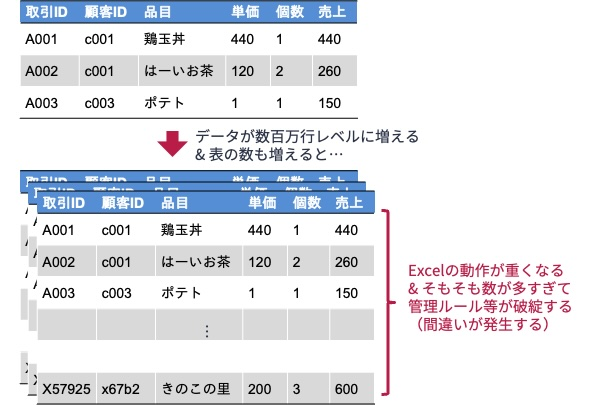
\includegraphics[width=1.0\textwidth]{figure/heavy-excel.jpg}
    \caption{管理する表データの規模や数が増えると破綻する.}
    \label{fig:heavy-excel}
\end{figure}


\subsubsection{データの正しさの保証}
管理するデータが大量かつ多様になってくると,データを正しく保つことが難しくなってくる.
管理対象となるデータに誤りが混入すると,大変なことになる.
例えば,図\ref{fig:bad-data}のように,購買データの中に
\begin{itemize}
\item 現実にはあり得ない売り上げ金額が記録されている
\item 入力形式が異なる日付が混在している
\item 取扱商品リストにないはずの商品が購買履歴に含まれている
\end{itemize}
といったことが起きると,オンラインショッピング事業においては一大事である.
それゆえ,データ管理においては,格納されるデータの正しさ,データ間の矛盾のなさを保証する機能が求められる.

\begin{figure}[tb]
    \centering
    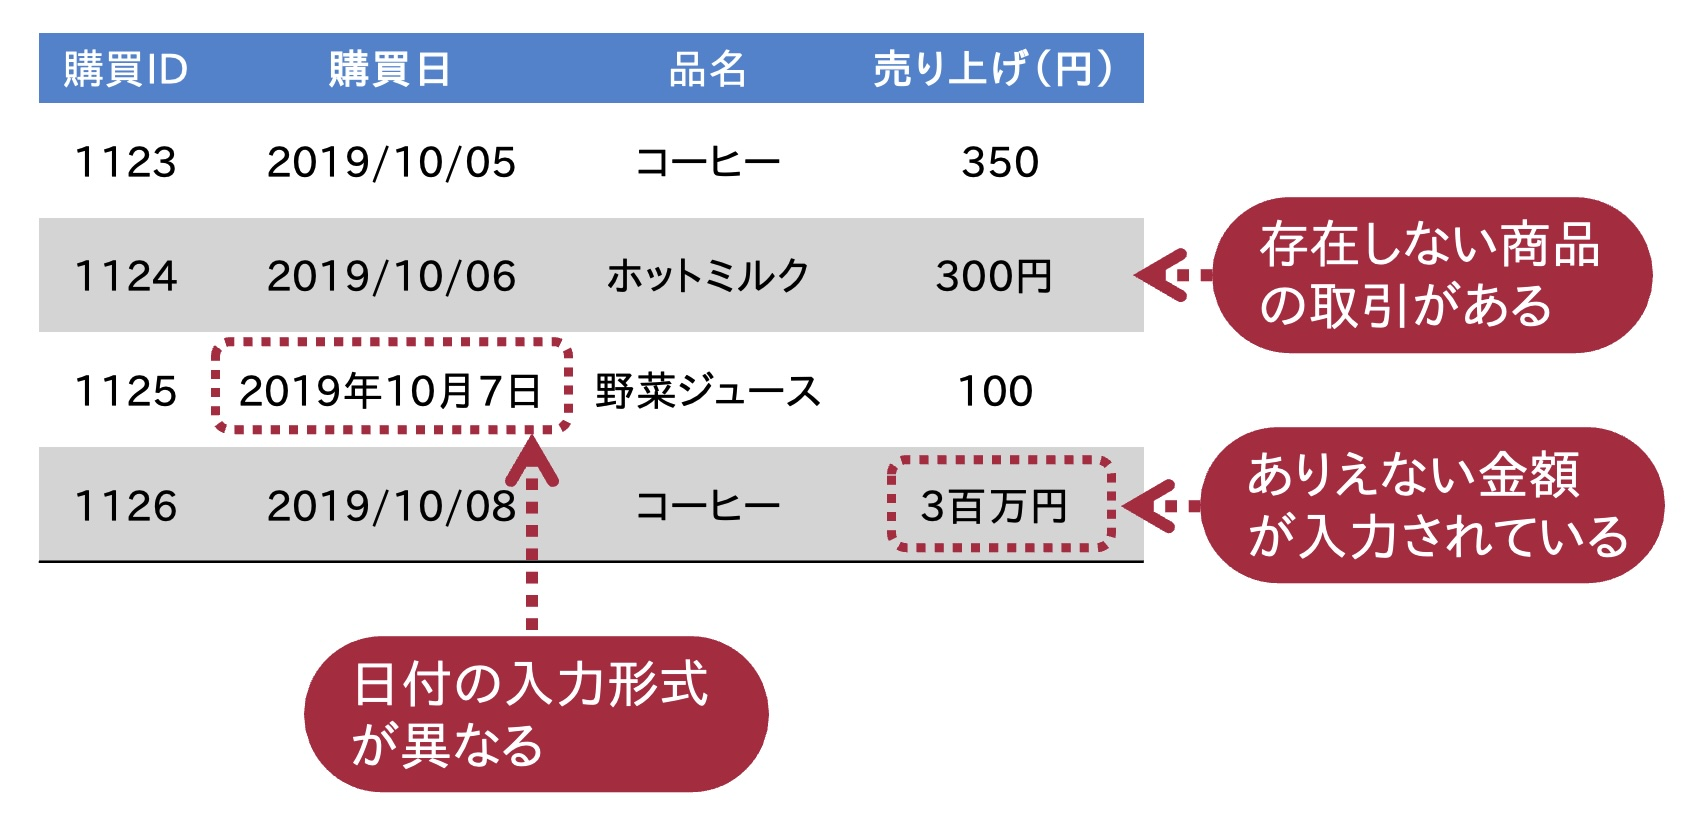
\includegraphics[width=1.0\textwidth]{figure/bad-data.jpg}
    \caption{バッドデータ(not ビッグデータ)の例.}
    \label{fig:bad-data}
\end{figure}


\subsubsection{高速で効率的なデータ処理}
データが大量に格納できたとしても,対象となるデータを高速に処理できなければ使い物にならない.
たとえ数百万件の書籍情報を格納しているシステムがあっても,ニーズを満たす書籍リストの検索結果を出力するのに数分待たされるようでは,そのようなシステムは使われない.

ユーザが増えるに従って,システムにかかる負荷も増える.
例えば,Amazon.co.jpでは毎分平均900件以上の商品取引が行われている\cite{TransactionInAmazon}.
このように大量のデータのやりとりが発生するケースにおいても,高速にデータ処理されることが求められる(図\ref{fig:linear-search-for-table}).

\begin{figure}[tb]
    \centering
    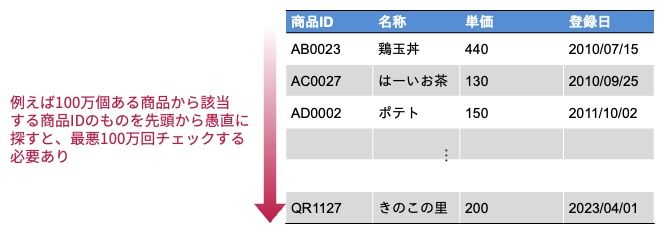
\includegraphics[width=1.0\textwidth]{figure/linear-search-for-table.jpg}
    \caption{線形探索では大規模データに対する高速なアクセスは難しい.}
    \label{fig:linear-search-for-table}
\end{figure}


\subsubsection{同時実行(並列処理)}
関連して,大勢の人が同時にデータを検索,追加,更新,削除しても,システムが問題なく動作することも重要である.

例えば,Xさん,Aさん,Bさんがとあるネット銀行の口座を利用しているとしよう.
Xさんの口座残高は100万円であるとする.
振り込みがあった際,振込先口座の残高の計算は
\begin{quotation}
残高 = 振り込み時の「振込先口座」の残高 + 振込額
\end{quotation}
振込元口座の残高の計算は
\begin{quotation}
残高 = 振り込み時の「振込元口座」の残高 - 振込額
\end{quotation}
となる.
これはは至極当然の処理であるが,次のような状況を考えてみよう.

ある日,AさんとBさんがXさんの口座に一秒の狂いもなく,\strong{まったく同時}に10万円送金したとする.
この際,前述の計算式をそのまま適用すると,図\ref{fig:mutual-exclusion}のように誤った処理が行われてしまう.
\begin{figure}[tb]
    \centering
    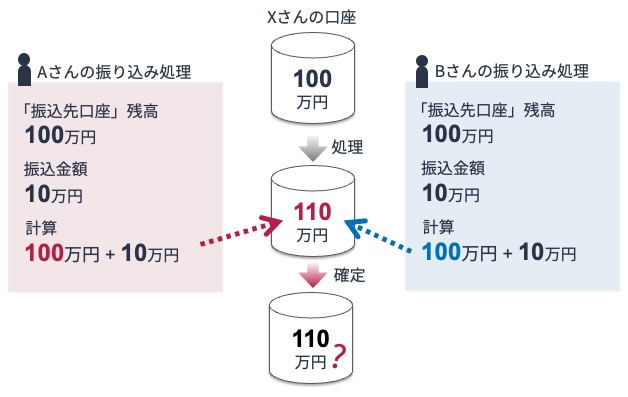
\includegraphics[width=0.9\textwidth]{figure/mutual-exclusion.jpg}
    \caption{複数の処理要求を矛盾なく処理できていない例.}
    \label{fig:mutual-exclusion}
\end{figure}
AさんとBさんが振込みを行った後,Xさんの口座の残高は110万円になりました -- こんなことが起きたら大変である.
この例における問題点は,たとえ振込み処理が同時に発生したとしても,Aさんの振り込み処理を待ってからBさんの処理を行うべきであったという点である.

このように,データ処理の内容によっては,別の処理が完了したことを保証してから次の処理を行う必要がある.
さらに,処理の途中で何らかのエラーが起きた場合は,すべての処理をキャンセルして最初の状態に戻すことが求められる.
同時にアクセスがあった場合でも,データを矛盾なく処理できることが重要である.


\subsubsection{アクセス権限のコントロール}
データによっては,誰でも自由に閲覧してよいものもあれば,特定の立場のユーザしかアクセスできないようにすべきものも存在する.
多種多様なデータのやりとりが発生する環境においては,ユーザの属性ごとにデータの閲覧,作成,更新,削除といったアクセス権限を制御する機能が必要となる.


% ---------------------------------------
\section{データベースを用いるメリット}
% ---------------------------------------
一人で扱えるほどデータの規模が小さければ,Excelなどの表計算用のソフトウェアでデータ管理しても問題はない.
しかし,扱うデータが多様かつ大規模になると,要求されるデータ処理の質が変わる.
そのため,データの管理方法や処理方法を見直す必要がある.

本稿で学ぶデータベースを用いれば,\strong{データの一元管理}が可能となり,データの管理や利活用において様々な恩恵を受けられる.
具体的には,データベースが備える以下のような特性あるいは関連技術を用いることで,前節で述べた「データ処理に求められる要件」をクリアすることができる.
\begin{itemize}
\item 大規模なデータの管理:「\strong{物理的データ格納方式}」の工夫によって対応
\item データの正しさの保証:「\strong{一貫性制約}」によって対応
\item 高速で効率的なデータ処理:「\strong{索引づけ}」「\strong{問い合わせ最適化}」などで対応
\item 同時実行,データの共同利用:「\strong{トランザクション}」などで対応
\item アクセス権のコントロール:「\strong{ロール管理}」によって対応
\end{itemize}


% ---------------------------------------
\section{データのモデリング}
% ---------------------------------------
\subsubsection{モデリングとは?}
科学やビジネスの世界では,モデルあるいはモデリングという用語がしばしば登場する.
ビジネスプロセスモデル,物理モデル,統計モデルなど,世の中には様々なモデルが存在する.
モデルとは,複雑な仕組みや現象,状態などを表現・分析・操作しやすくするために,本質的でない要素を取り除き,関心のある側面のみを抽出し抽象化したものである.
\strong{モデリング}とはモデル化,つまりモデルを作る行為である.


\subsubsection{データモデリング}
データベースで何らかのデータを扱う場合,まずデータをモデリングする.
世の中に存在するデータは多種多様であり,データを統一的に整理し,計算機で処理しやすい形に抽象化,すなわちモデリングする必要がある.

\strong{データモデリング}とは,データベース化すべき情報を取捨選択し,対象とするデータとその操作に関する枠組み(\strong{データモデル; data model})を設計する行為である.
対象とする事象やアプリケーションに応じて適切なデータモデルを設計することで,データモデルに従って実データを格納し,操作することが可能となる.

一般に,データモデルは以下の3つの要素を含む:
\begin{itemize}
\item データの構造
\item データの制約条件
\item データの操作
\end{itemize}

本講義の主要テーマである\strong{関係データベース(relational database)}は,\strong{関係データモデル(relational data model)}\footnote{関係モデル(relational model)と呼ぶこともある.}に基づき設計されたデータベースである.
関係データモデルの詳細については,次章で説明する.

データベース管理システムで扱われるデータモデルとしては,関係データモデルのほかにも以下のようなものがある:
\begin{itemize}
\item ネットワークモデル\cite{Bachman1969}
\item 階層型データモデル\cite{Tsichritzis1976}
\item オブジェクト指向モデル\cite{Atkinson1994}
\item キー・バリュー(key-value)モデル\cite{DeCandia2007}
\item グラフデータモデル\cite{neo4j}
\end{itemize}

% ---------------------------------------
\section{関係データモデル(導入)}
% ---------------------------------------
関係データモデルは,最も代表的なデータモデルである.
1970年にEdgar F. Codd氏により提案されたもので,単純ながらその背後には強力な数学的基盤をもつ\cite{Codd1970}.
関係データモデルでは,あらゆるデータを\strong{表(table)}としてモデル化する.

図\ref{fig:example-of-relation}は,関係データモデルを用いて構築された,授業の履修状況・成績を管理する関係データベースの例である.
この関係データベースには,以下の3つの表\footnote{テーブルと呼ぶこともある.}が存在する.
\begin{itemize}
\item 学生テーブル:学籍番号,氏名,入学年度,所属といった学生に関する情報を格納
\item 科目テーブル:科目ID,科目名,開講年度といった科目に関する情報を格納
\item 履修テーブル:どの学生が何の科目を履修し,どのような成績であったかに関する情報を格納
\end{itemize}

\begin{figure}[tb]
    \centering
    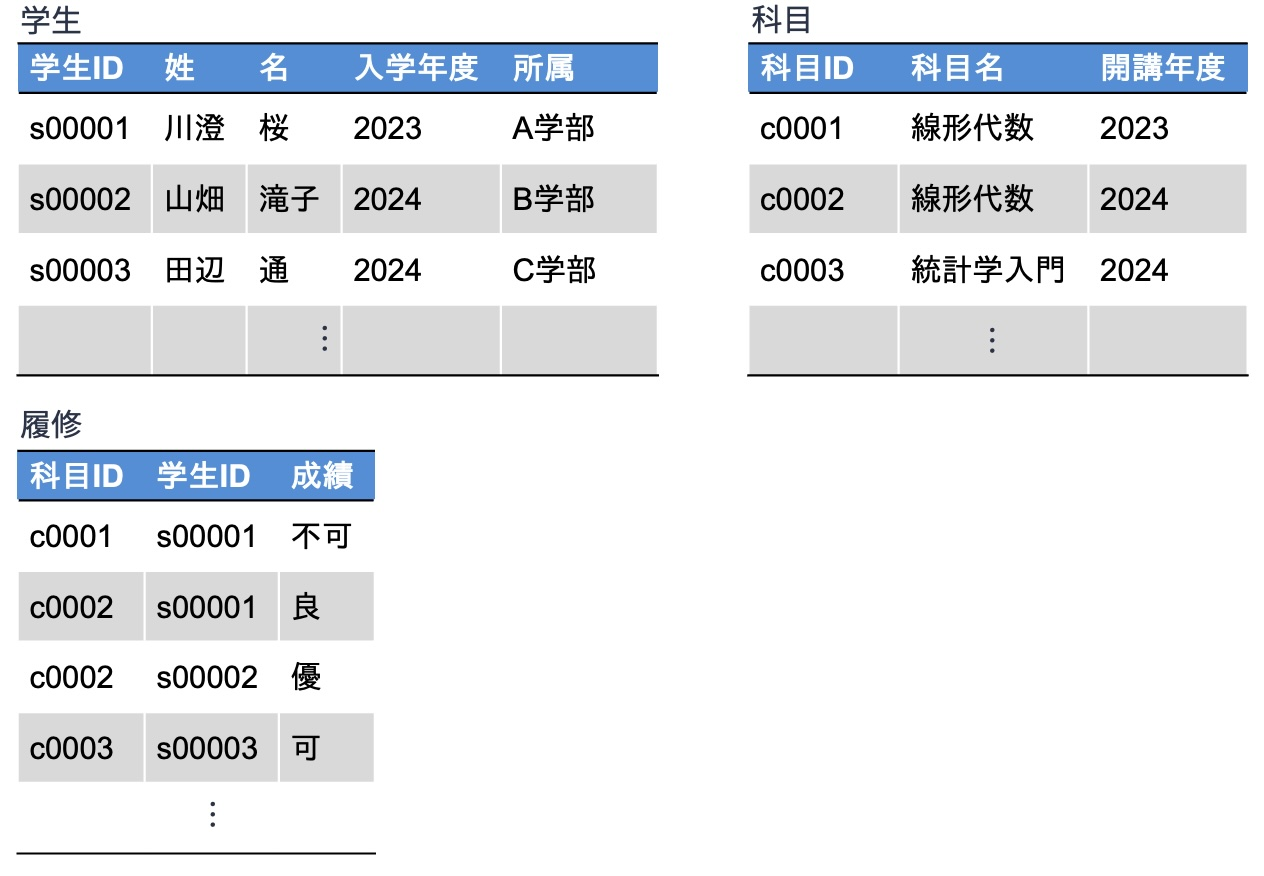
\includegraphics[width=1.0\textwidth]{figure/example-of-relation.jpg}
    \caption{関係データベースの例.}
    \label{fig:example-of-relation}
\end{figure}
この例だけ見ると「なんだ,関係データモデルとは単なる表なのか」と思われたかもしれないが,\strong{ただの表ではない}.
関係データモデルに基づいて表現された(表)データは,あらかじめ定義された「データの構造」「データの制約」「データの操作」に関する規則に従ってデータが作られ,関係データベース内に格納される.
例えば,以下のような規則が考えられる:
\begin{itemize}
\item 学生テーブルは「学生ID」「姓」「名」「入学年度」「所属」という見出しをもつ
\item 履修テーブルには,科目名や学生の氏名を格納しない
\item 履修テーブルの成績には「優」「良」「可」「不可」のいずれかしか登録できない
\item 履修テーブルに現れる科目IDおよび学生IDは,必ず学生テーブルと科目テーブルに存在する
\item 学生テーブル,科目テーブルの各テーブルにおいて,同じ科目IDは存在しない
\end{itemize}
このような規則に従い,授業の履修状況や成績を管理するための情報が,複数のテーブルに分割され格納される.

次章以降では,
\begin{itemize}
\item このような規則,すなわち関係データモデルをどう設計するのか
\item 一見ただの表にしか見えない関係データモデルが,どのように数学的に定式化されているか
\item 関係データモデルを用いると,なぜ大規模データの管理が効率的になるのか
\end{itemize}
などについて詳しく述べていく.

% ---------------------------------------
\section{クイズ}
% ---------------------------------------
\subsubsection{Q1. メジャーなデータベース管理システム}
ウェブ検索エンジンを用いて,世の中にあるメジャーなデータベース管理システムを調べなさい.
また,調べたデータベース管理システムを「関係データベースを扱うもの」と「そうでないもの」に分類せよ.

\subsubsection{Q2. 線形探索}
100万件ある商品リストの中に特定の商品が含まれているかを確認したい.
商品リストの先頭から末尾まで順に商品名を確認していくと,平均で何回(何件)の確認で商品の有無を確認できるか?

\subsubsection{Q3. データベース管理システムの利用例}
普段利用しているサービスのうち,データベース管理システムを用いていると思われるものを3つピックアップしなさい.

\subsubsection{Q4. CSV/TSVファイル}
CSVファイルおよびTSVファイルとは何かを調べなさい.
また,(データベース管理システムでデータを管理する場合と比較して)CSV/TSVファイルに存在する欠点を挙げなさい.

\subsubsection{Q5. チューリング賞}
関係データモデルを提唱したEdgar F. Codd氏は,計算機科学分野のノーベル賞といわれるチューリング賞の受賞者である.
Codd氏以外で,データベースに関する功績でチューリング賞を受賞した人をピックアップしなさい.
